\makeatletter
\def\input@path{{../}}
\makeatother

\documentclass[/main.tex]{subfiles}
\graphicspath{{./pics/}{appEventBuilder/pics/}}
\begin{document}

\onlyinsubfile{\appendix}
\chapter{The \MJD\ Event Builder}
\label{app:eventbuilder}

The primary purpose of the \textsc{Majorana Demonstrator}'s event builder is to convert raw data files produced by ORCA into built files to be used in the next stages of analysis.
Built files use the .root file format, which is compatible with the root analysis framework.
Data is stored in these files as data objects from the \textsc{Majorana Gerda} Data Objects (MGDO) library.
The data is stored as events, which contain multiple waveforms and associated digitizer data such as energy and time that take place close together.
The event builder is responsible for combining individual data packets into events.
In addition, the event builder performs many basic data quality checks, or garbage checks.

\section{Built File Contents} \label{sec:file_contents}

A built file is a ROOT file, which is written and read by the ROOT analysis framework.
ROOT files offer several advantages for storing large quantities of data: they enable relatively simple interfacing with \cpp libraries, they are robust under schema evolution, and they handle data compression automatically.
Data is stored primarily in TTrees, which are buffers containing a large number of same-class \cpp objects.
The contents of the MJD built files will be described in this section.

\begin{description}
\item[MGTree:] A TTree containing Germanium detector data. The tree has the following two branches:
  \begin{description}
  \item[run] contains MJTRun objects which hold basic run data such as run number and start and stop times.
  \item[event] contains MGTEvent objects, which contain the individual waveforms and associated digitizer data and data about the event as a whole.
  \end{description}

\item[MGGarbageTree:] A TTree containing Germanium detector data that has failed data quality checks. The tree has the following three branches:
  \begin{description}
  \item[run] contains MJTRun objects which hold basic run data such as run number and start and stop times.
  \item[event] contains MGTEvent objects, which contain the individual waveforms and associated digitizer data and data about the event as a whole.
  \item[garbageCode] is a 32-bit mask encoding which garbage checks failed. The meaning of each bit is in section \ref{sec:garbage_bits}
  \end{description}

\item[VetoTree:] A TTree containing veto data from the CaenV830Scaler card and Caen792Nqdc cards. The tree has the following 4 branches:
  \begin{description}
  \item[run] contains MJTRun objects which hold basic run data such as run number and start and stop times.
  \item[vetoEvent] contains MGTBasicEvent objects, which detector data from one scaler data packet and several Nqdc data packets.
  \item[mVeto] contains the event multiplicity, which is the number of QDC channels above threshold.
  \item[vetoBits] contains a 32-bit mask encoding the results of several checks described in section \ref{sec:veto_bits}
  \end{description}

\item[headerXML:] A string of the XML header from the ORCA file. This contains information about the run configuration and is formatted as an XML plist.
  
\item[ChannelMap:] A MJTChannelMap object, compiling information from the tables in the MajoranaModel ORCA object, which describe which detector, pulser, and array position corresponds to each channel. This is useful for obtaining information about each channel, such as detector name and position. The channel map uses a table structure with one row for each Germanium detector.
  
\item[ChannelSettings:] A MJTChannelSettings object. This contains information about the settings for each card. These settings are stored as a tree, with a node hierarchy of card name$\rightarrow$ crate $\rightarrow$ card $\rightarrow$ setting name $\rightarrow$ channel.

\item[builderInfo:] A string containing information about how the file was built. It contains the command used to build the file and information about the version of MJOR and its dependancies.
  
\end{description}



\section{Code Structure}
MJOR is based on OrcaRoot, an object-oriented \cpp library designed to process an ORCA data stream into a ROOT data structure, typically a TTree.
OrcaRoot reads out one data packet at a time using either the ORFileReader or ORSocketReader classes.
A data processor manager (class ORDataProcManager) passes each data packet to data processor classes (inheriting from ORDataProcessor).
MJOR contains data processors for the various data readout cards used by the \textsc{Majorana Demonstrator} and data processors for combining data into events and writing events to TTrees.
The majorcaroot executable is used to setup the data loaders that will be used for an ORCA datastream.
This section will describe the majorcaroot executable and the various data processor classes.

\subsection{majorcaroot}
majorcaroot is the executable used to run the event builder.
The command line options are described in section \ref{sec:majorcaroot_options}.
majorcaroot process each file twice.
On the first pass, only the ORRunTimesCalculator is used, which only processes the run stop packet in order to find the end time of the run, as recorded by ORCA, and the total number of data packets in the run.
After this, the run is processed again, with the processors handling the detector data.
\par
When processing the data the second time, the data processor MOHeaderProcessor is used.
MOHeaderProcessor inherits from ORHeaderProcessor, which reads the XML header from the ORCA datastream.
MOHeaderProcessor also edits the XML header, if certain command line options are used.
For example, the run type can be changed or a special channel map can be added.

\subsection{Germanium digitizer processors} \label{sec:EB_description}
The event builder is represented by the class class MOEventBuilder, which is the data processor responsible for building Germanium detector events.
The data loader is represented by the class MOEventDataLoader and daughter classes MOGretina4MDataLoader, MOGretina4DataLoader, and MOSIS3302DataLoader, which are data processors responsible for reading the waveforms and digitizer data out of the data stream.
A flow diagram of the Germanium data loader and event builder is shown in figure \ref{fig:EB_diagram}.
\par
At the start of the ORCA datastream, the event builder allocates the data structures described in the following paragraphs.
It creates the branches in MGTree and MGGarbageTree, as described in section \ref{sec:file_contents}.
It also fills channel map with the contents of the tables in the MajoranaModel section of the XML header, and the channel settings with the contents of the hardware dictionary produced by OrcaRoot.
Finally, it fills the MJTRun, using the stop time and packet number found by the ORRunTimesCalculator.
If either the datastream is not an ORCA file or the file contains no run stop packet, the stop time and packet number are set to zero.
\par

\begin{figure}
  \centering
  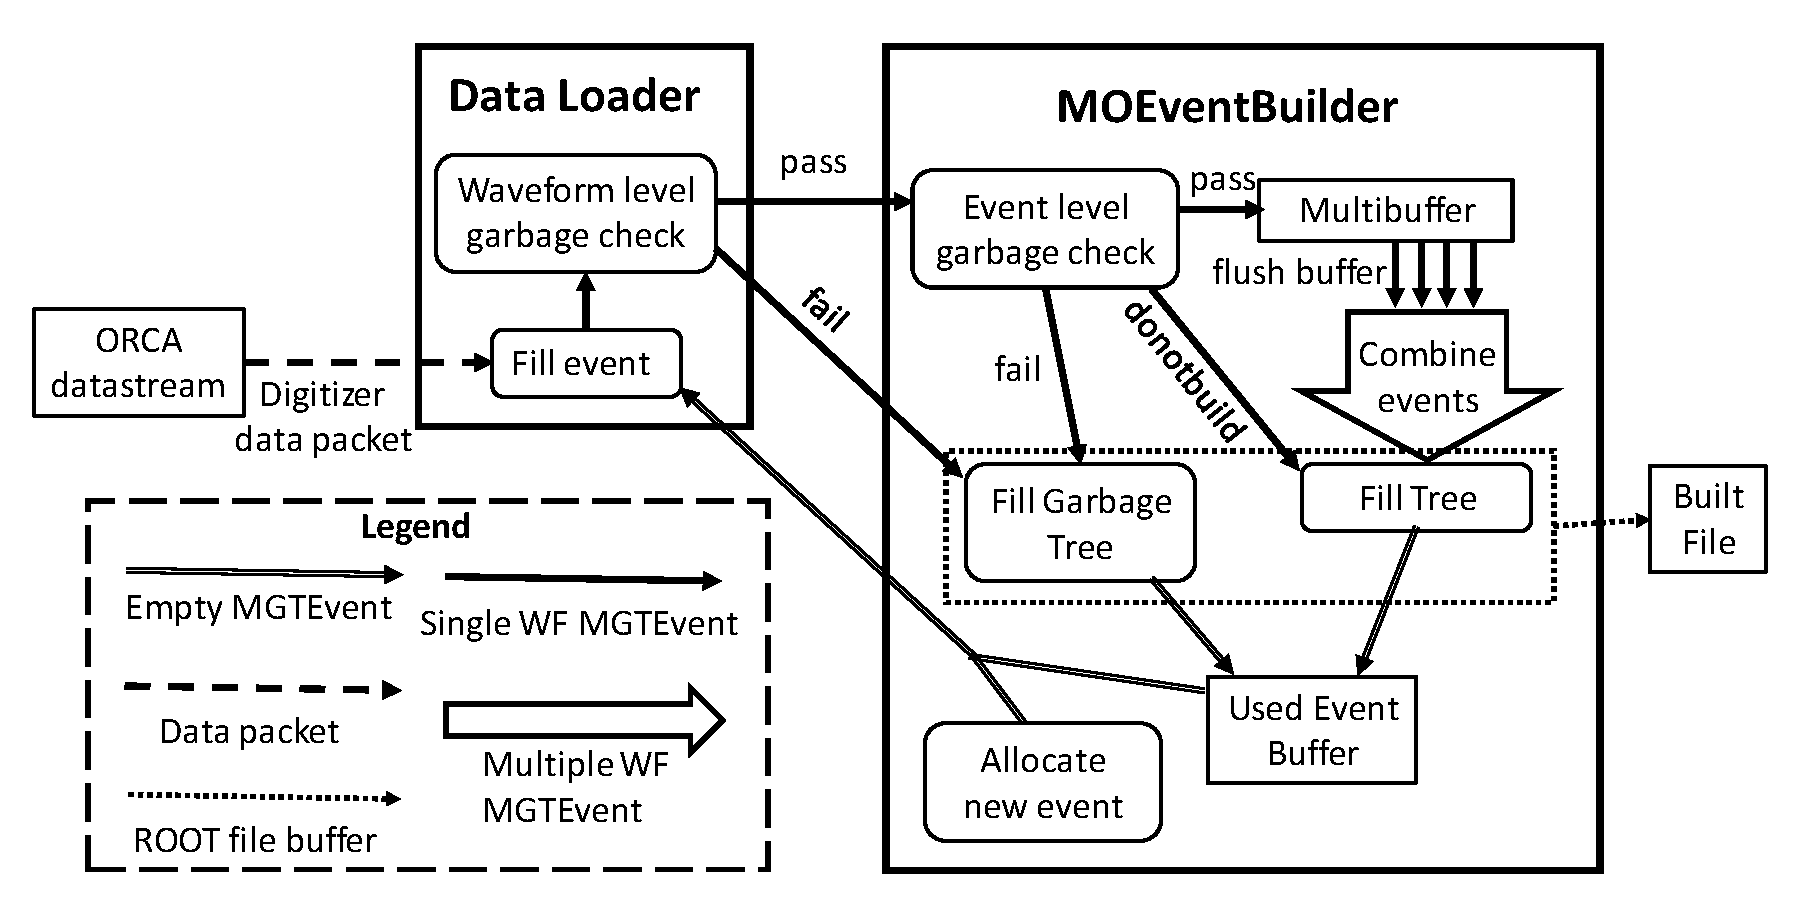
\includegraphics[width=.9\textwidth]{EventBuilderDiagram}
  \caption[Event builder data flow diagram]{\label{fig:EB_diagram}
    Data flow diagram for building Germanium events as described in section \ref{sec:EB_description}. The logic for flushing the buffer is layed out in figure \ref{fig:MB_diagram}}
\end{figure}

When a digitized waveform is read from the ORCA datastream, the data loader class requests an empty event from MOEventBuilder, which will be popped from a buffer of used, empty events called the used event buffer.
If the used event buffer is empty, a new event is allocated instead.
The purpose of the used event buffer is to recycle the waveform objects and avoid repeatedly allocating and deallocating large arrays.
The data loader class fills the empty event with a single MGTWaveform and MGTGretina4DigitizerData object, filled using the data packet from ORCA.
The data loader then performs waveform level garbage checks for data corruption that can be detected within a single data packet.
The event is then passed to the event builder.
\par
The event builder does one of three things with the new event.
If the event was flagged as garbage, it is immediately recorded into MGGarbageTree, cleared, and recycled into the used event buffer.
If the event builder is run in donotbuild mode, the event is immediately recorded into MGTree, cleared, and recycled into the used event buffer.
Otherwise, the event is placed into the multibuffer, a \cpp standard library map from a channel number to a \cpp standard library vector of single-waveform events.
The multi-buffer structure is used because data packets from within a single channel are time-ordered, but packets across multiple channels are not.
Thus, this structure does not require sorting events by timestamp and it makes timestamp-based garbage checks much simpler to implement.
Before being added to the multibuffer, event-level garbage checks are performed, which require comparing multiple waveforms and digitizer data.
If these checks fail, the event is not recorded into the multi-buffer, but instead is immediately written to the garbage tree, cleared, and recycled into the used event buffer.
Otherwise, the event is placed into the buffer for its channel and the event builder checks whether or not to flush the oldest event from the multi-buffer.
\par
The event buffer has two possible conditions for flushing the buffer.
First, if all channels have at least two events, the buffer will flush.
This condition is chosen because once every buffer has at least one event, no more waveforms should appear with a timestamp earlier than any waveforms presently in the buffer.
In order to ensure that the event builder can continue to make event level garbage checks, it is important that each buffer is left with at least one event, so the condition is two events in each channel instead of one.
The second condition for flushing the buffer is when the buffer has too many events or uses too much memory.
The exact condition can be changed by selecting the correct command line option.
The default option is to flush when 10000 events are in the multi-buffer.
This second condition should only be needed if one channel has a significantly lower data rate than the others, causing the multibuffer to fill up.
The buffer is flushed by merging any events within the time window into a single built event.
Events are merged by moving the waveform and digitizer data into the built event.
The merged event is then cleared and recycled into the used event buffer.
If an event is merged with a timestamp later than the latest timestamp in the event, the event window is expanded and any waveforms in the new window are merged into the event.
After the built event has been filled, event parameters such as the oldest timestamp and total energy of the event are set.
Finally, the event is written to MGTree, cleared, and recycled into the used event buffer.
\par

\begin{figure}
  \centering
  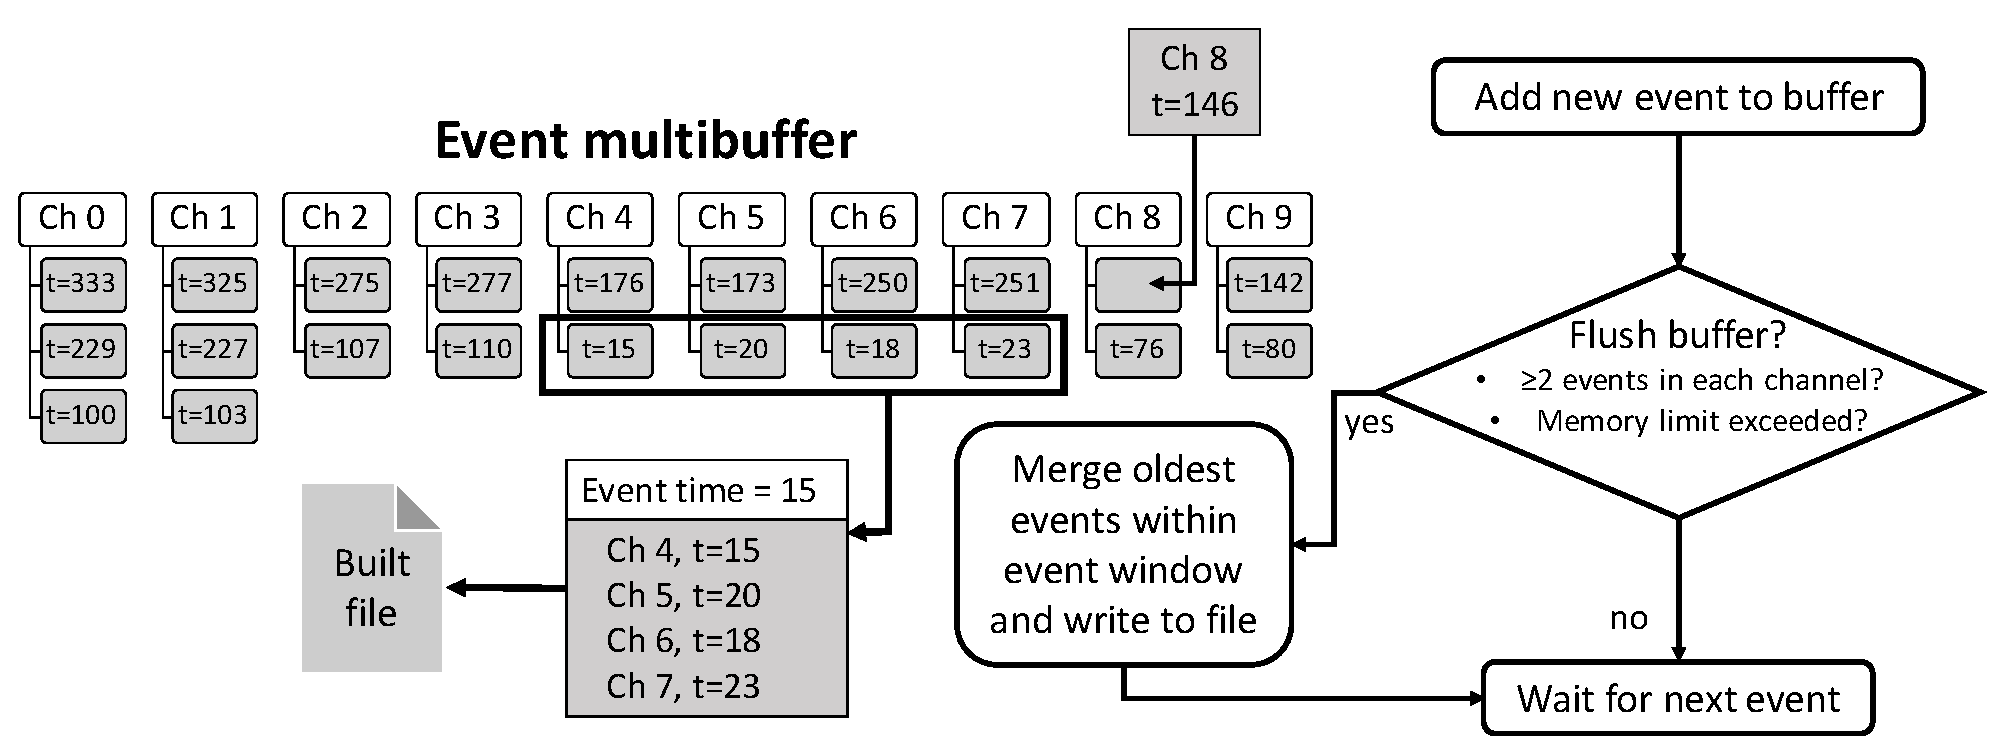
\includegraphics[width=0.9\textwidth]{MultibufferDiagram}
  \caption[Event builder multibuffer diagram]{\label{fig:MB_diagram}
    Diagram of multibuffer structure and logic for flushing events from buffer, as desribed in section \ref{sec:EB_description}.}
\end{figure}

This scheme for flushing the multibuffer can lead to misbuilt events under two conditions.
First, if the data rate is very high in at least one channel and very low in another, the high rate channels can trigger the second condition and flush an event with a timestamp later than a waveform in the low rate channel that has not yet been read into the buffer.
In this case, the low rate channel waveform will be written into the garbage tree.
The data rates in MJD's collaboration runs are not high enough to trigger this under ordinary circumstances.
If this does become a problem, it can be reduced by increasing the threshold for flushing the buffer due to memory or event count.
The second cause of misbuilt events is when the data rate is high enough in enough channels that the sliding event window expands multiple times and includes a waveform from a channel that has already appeared in the event.
Ordinary data rates in MJD calibration runs are not high enough to cause this to occur.
This can be made less likely by reducing the event window, which defaults to 10~$\mu$s

\par
Once the entire ORCA datastream has been read by the event builder, any events remaining in the multibuffer are merged and written to MGTree.
Finally, MGTree, MGGarbageTree, and the channel map and settings are written to the built file.

\subsection{Veto processors} \label{sec:veto_description}
The data processors MOCaen792NqdcDataLoader and MOCaenV830DataLoader are used to read data from the QDC and scaler cards, respectively.
The class MOVetoDataLoader combines the data from both of these processors into MGTBasicEvents and writes these events into VetoTree.
A dataflow diagram for the veto loader is shown in figure \ref{fig:veto_diagram}.
The expected ordering of data packets in the ORCA data stream for a veto event is a scaler data packet followed immediately by a QDC packet for each QDC card.
No other data packets are expected between any of these.
The veto loader is written with the expectation that data packets appear in this order.
\par
At the start of the ORCA datastream, VetoTree is initialized and its branches are created as described in section \ref{sec:file_contents}.
The MJTRun is filled, using the ORRunTimesCalculator as described in the previous section.
A single MGTBasicEvent is allocated to act as a buffer for the veto data.
\par
Whenever a scaler data packet is read by the ORCA datastream, the data is stored by the MOCaenV830DataLoader class.
The data from only a single scaler packet is stored at any given time, and should always consist of the most recently read scaler packet.
When a QDC data packet is read, the data from each channel is put into its own MJTVetoDetectorData object along with the currently stored scaler data.
Each detector data is placed into the MGTBasicEvent buffer.
Every time a scaler data packet is read, the MOVetoDataLoader class writes the event buffer to VetoTree and clears the event.
In this way, each QDC packet is associated with the most recent scaler packet, as expected for the ordering of data packets described at the start of this section.
Before writing the event, several basic data checks, described in section \ref{sec:veto_bits}, are performed and the vetoBits bitmask is set.
\par
At the end of the ORCA datastream, the remaining data is written to VetoTree, and VetoTree is written to the built file.


\begin{figure} 
  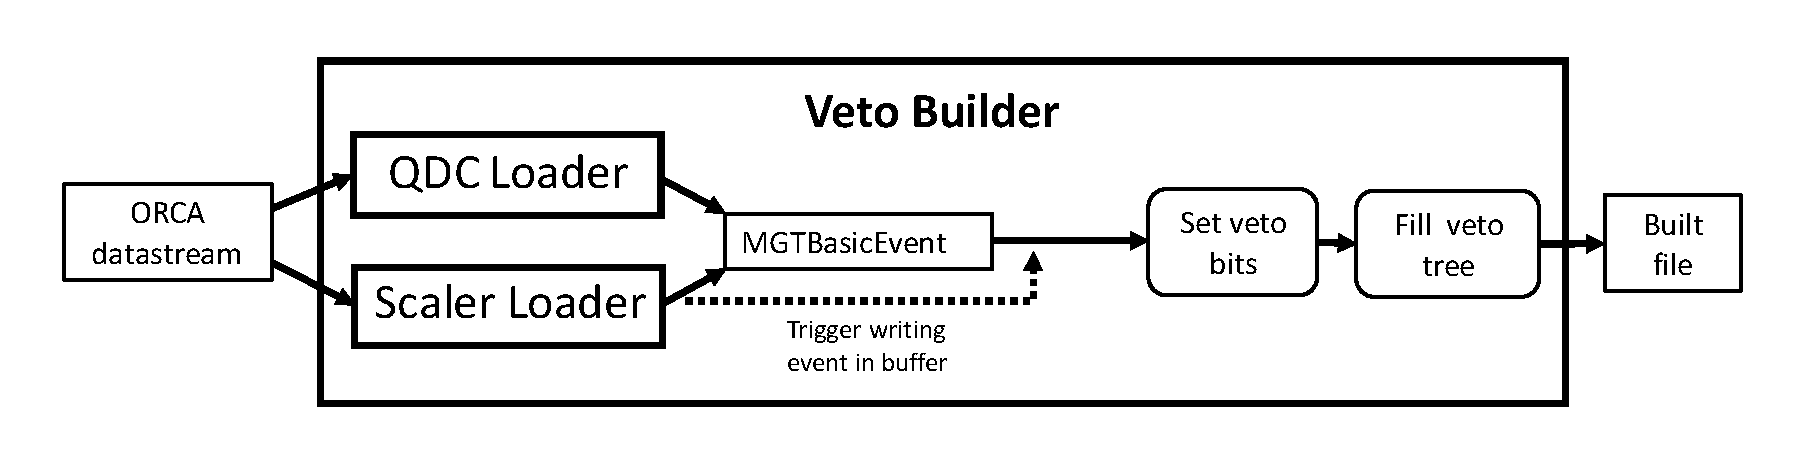
\includegraphics[width=0.9\textwidth]{VetoBuilderDiagram}
  \caption[Diagram of data flow for building veto events]{\label{fig:veto_diagram}
    Data flow diagram for building Germanium events as described in section \ref{sec:veto_description}.}
\end{figure}

\subsection{majorcaroot usage and options} \label{sec:majorcaroot_options}
majorcaroot can be called either on a set of raw ORCA files or on a port of a socket.
The correct usage is \texttt{majorcaroot [options] [input file(s)/socket host:port]}.
The possible options are:

\begin{description}
  \item[-h, --help] : print a usage message and exit
  \item[-v, --verbosity [verbosity]] : set the severity/verbosity for the logger. Choices are: debug, trace, routine, warning, error, and fatal.
  \item[-t, --eventwindow [time]] : set the windowing time for the event building. Format is [number][unit] (no space). Unit choices are s, ms, us, ns. If not specified, majorcaroot uses "10us". 
  \item[-x, --disablevalidatexml] : do not validate the XML plist in the ORCA file header. ORXmlPlist will generate a warning. Use when not online.
  \item[-e, --nevents [num]] : Only process until nevents are in the output tree. 
  \item[-s, --sis] : use SIS3302 data loader. 
  \item[-g, --gret] : use Gretina4 data loader. 
  \item[-G, --gretM] : use Gretina4M data loader.
    \\By default, majorcaroot will look into XML header to check which data loader to use.
  \item[--veto [on/off/qdconly/donotbuild]] : force veto loader on or off. Default is to turn on if both Caen 792 Nqdc and Caen V830 scaler data are found. Use qdconly if scaler card is not in use but qdc card is. donotbuild will write veto events whenever a qdc data packet is encountered, meaning events only will contain data from a single qdc packet.
  \item[-n --nomca] : do not use data builder for ORTEC 927 MCA even if MCA data exists. 
  \item[-i, --mangleChannelIDsForGELATIO [num]] : subtract the [num] from all crate-card-channel IDs (dangerous; for GELATIO users). 
  \item[-C, --disablecollectgarbage] : do not throw away bad events into MGGarbageTree.
  \item[-f, --fixheaderbools] : fix booleans in XML header that have been stored incorrectly by ORCA. This is only necessary for older versions of ORCA.
  \item[-r, --setrunbits [bits]] : Set run type bits to the given value. Can be given in decimal or hexidecimal with prefix 0x.
  \item[--forcerunbitson [bits]] : Turn on all bits set to 1 and ignore bits set to zero. Can be used in combination with --forcerunbitsoff.
  \item[--forcerunbitsoff [bits]] : Turn off all bits set to 1 and ignore bits set to zero. Can be used in combination with --forcerunbitson
  \item[--setspecialchanmap [name of file] : Set the special channel map to the contents of a file.
  \item[-D, --donotbuild] : push events to the output tree for each digitizer record: do no time sorting or event clustering. 
  \item[-E, --doubleencoding] : use double encoding instead of short. This results in a larger file size. 
  \item[-I, --ignoreenabled] : do not check for bad channels. Do not flush buffer when all enabled channels have events. This is for debugging purposes only.
  \item[-N, --limbufevents [num]] : flush buffer when it contains more than [num] events. 
  \item[-T, --limbuftime [time] : flush buffer when it contains events older than [time] relative to incoming events. 
  \item[-M, --limbufmem [MB]] : flush buffer when it grows larger than [MB] megabytes ([MB] should be an int). 
  \item[-P, --limbufmempct [pct]] : flush buffer when it grows larger than [pct] percent of the system memory (integer between 1 and 100). \\
    Default limbuf method is equivalent to --limbufevents 10000.
\end{description}

\subsection{majorcaroot\_checker}
The majorcaroot\_checker program checks a single built file to ensure that they are built correctly.
The correct usage is \texttt{majorcaroot\_checker [built file]}.
majorcaroot\_checker accepts no options; instead, it reads the builderInfo string from the built file in order to determine which options to use.
majorcaroot\_checker is not guaranteed to correctly check files that originated with majorcaroot from a different version of MJOR.
\par
majorcaroot\_checker begins by looping through each of the TTrees in the file and performing several checks on each event.
A list is allocated with size equal to the total number of data packets in the run in order to count the number of properly built events in each data packet.
If an event fails checks performed on it, then it is not added to this list.
\par
In MGTree, each event is checked to ensure that it is in order by time and that each waveform falls in the correct time window.
The event is also checked to ensure that each channel does not have multiple waveforms.
Finally, each waveform is checked to ensure that all MGTWaveform data members were filled and do not contain corrupt data.
\par
In MGGarbageTree, specific checks are not performed on waveforms since any problems are assumed to be related to the reason the waveform is in MGGarbageTree to begin with.
If the garbageCode indicates a corrupt data header or bad timestamp and the event occurred in the middle of a run, a warning is emitted, since these types of garbage events are common at the start and end of runs, but not in the middle.
After scanning through the tree, majorcaroot\_checker outputs a list of each unique set of garbage bits in the tree, and how many times they occurred.
\par
In VetoTree, each veto event is checked to ensure that all data members are filled correctly.
After scanning through the tree, majorcaroot\_checker outputs a list of each unique set of veto bits in the tree, and how many times they occurred.
\par
After scanning each tree, the checker rescans the original ORCA file, assuming that the original file has the same relative path as when majorcaroot was first run.
The checker scans using the MOOrcaFileFilter data processor.
This processor takes the list of built data packets that was filled while scanning each tree as an input.
For each data packet that is not found in the list or has the wrong number of entries (e.g. if a gretina data packet has 8 entries, but only 7 were found in MGTree with the correct index), the raw data record is written into a new ORCA binary file.
Furthermore, a count of the number of data packets from each type of card in the file is given.





\section{Bit Definitions}
This section contains the definitions of garbage bits, run bits, and veto bits.
These bits are stored as 32-bit masks, with each bit representing some condition.
Multiple bits may be set at once.
The bits are listed in tables from least significant bit to most significant bit, with double lines breaking up hexadecimal digits.
The bits are defined in MGDO in the header file Majorana/MJTypes.hh, along with some basic commands for manipulating them.

\subsection{Run bits} \label{sec:run_bits}
The run bits are contained in the XML header of the ORCA file and are read into the run branch of each tree.
These bits are set during ORCA run configuration, however options exist to change these bits in the built file.
\par
\begin{tabular}{| l | l | p{0.6\textwidth} |} \hline
  bit & name & description \\ \hline\hline
  0  & Maintenance           & This is already defined. It is tied to the operations in ORCA and is used when the operator is making changes, etc. to the configuration \\ \hline
  1  & bb-decay              & Selected for "good" data taking. \\ \hline
  2  & Calibration-Prototype & Set if calibration source present on Prototype. \\ \hline
  3  & Calibration-Module 1  & Set if calibration source present	
  on Module 1. \\ \hline\hline
  4  & Calibration-Module 2  & Set if calibration source present on Module 2. \\ \hline
  5  & Co60                  & Set for use of Cobalt-60 source. \\ \hline
  6  & Th228                 & Set for use of Th-228 source. \\ \hline
  7  & Partial shield        & Set if part of poly shield is not present. \\ \hline\hline
  8  & Prototype offline     & Set if Prototype is offline. \\ \hline
  9  & Module 1 offline      & Set if Module 1 is offline. \\ \hline
  10 & Module 2 offline      & Set if Module 2 is offline. \\ \hline
  11 & Radon purge offline   & Set if radon purge is offline or abnormal. \\ \hline\hline
  12 & Machine shop          & Set if work ongoing in machine shop. \\ \hline
  13 & Disruptive work       & Set if work in Detector Room might be disruptive to data taking \\ \hline
  14 & Blank Monolith (East side) & Set if blank monolith is in east shield spot. \\ \hline
  15 & Blank Monolith (South side)& Set if blank monolith is in south shield spot. \\ \hline
\end{tabular}
\par
\subsection{Garbage bits} \label{sec:garbage_bits}
The garbage bits are encoded in the MGGarbageTree branch ``garbageCode.'' Each entry in MGGarbageTree should have an event with a single waveform/digitizer data and a non-zero garbage code.
The first three bits are specific to the Gretina4M card/firmware and will not be thrown for others.
The remaining bits will be thrown for any card/firmware.
\par
\begin{tabular}{| l | l | p{0.7\textwidth} |} \hline
  bit & name & description \\ \hline\hline
  0  & BadHeader1     & The first word of a Gretina4M data packet is not 0xAAAAAAAA \\ \hline
  1  & BadHeader2     & The second word of a Gretina4M data packet is not 0x000000D\#, where \# is any hexidecimal digit \\ \hline
  2  & BadHeader3     & The energy and timestamp in the Gretina packet header are both zero \\ \hline
  3  & TooOld         & Waveform has a timestamp older than an event that has already be written. This may indicate that the memory limits are too stringent.  \\ \hline\hline
  4  & InvalidCard    & Waveform comes from a card that is not being read out by ORCA \\ \hline
  5  & InvalidChannel & Waveform comes from a channel that is not enabled  \\ \hline
  6  & TSOutOfOrder   & Waveforms within a single channel should be time ordered. If a waveform comes after a waveform in the same channel with a later timestamp, set this bit. \\ \hline
  7  & RepeatWF       & Two consecutive waveforms within a single channel have identical waveforms \\ \hline\hline
  8  & NWaveforms     & Event contains no waveforms. This case represents an exception to garbage events having one waveform \\ \hline
  9  & AllZero        & Waveform has all zero entries \\ \hline
\end{tabular}
\par

\subsection{Veto bits} \label{sec:veto_bits}
Veto bits are assigned to each veto event in VetoTree.
The veto bits represont differences in veto events from the expected configuration.
Events that are tagged are not separated from normal events, meaning that the veto bits can be set to zero.
\par
\begin{tabular}{| l | l | p{0.7\textwidth} |} \hline
  bit & name & description \\ \hline\hline
  0  & MissingChannels  & \textless32 veto data objects exist in the event. \\ \hline
  1  & ExtraChannels    & \textgreater32 veto data objects exist in the event. \\ \hline
  2  & ScalerOnly       & Event has no QDC data. The event should contain a single veto-data with only have time and scaler-related fields set. \\ \hline
  3  & BadTimeStamp     & Timestamp is 0xFFFF FFFF FFFF FFFF.  \\ \hline\hline
  4  & QDCOutOfSequence & Event does not have the expected Scaler-QDC-QDC sequence. This is set if fQDCIndex - fScalerIndex is not 1 or 2.\\ \hline
  5  & DuplicateChannel & A QDC channel appears multiple times in a single event. \\ \hline
  6  & HWCountMismatch  & Event count on scaler changes from event count of QDC. This is only set for the event where the mismatch occurs.\\ \hline
\end{tabular}


\end{document}
